\documentclass[../main.tex]{subfiles}
\begin{document}
    Combien de petit carrés permettent de recouvrir le rectangle
    ci-dessous~?
    \begin{center}
        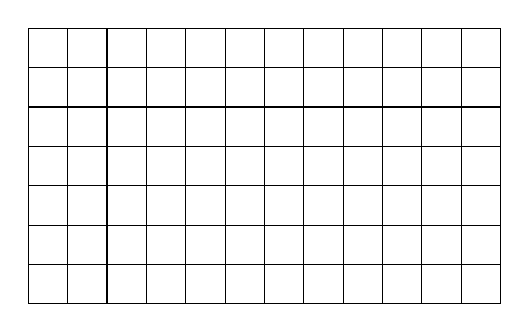
\begin{tikzpicture}[scale=0.5]
            \draw(0,0)grid(12,7);
        \end{tikzpicture}
    \end{center}
    \begin{simplebox}
        \textbf{Définition :} $1\;m^2$ (\guillemets{un mètre carré}) est l'aire d'un
        carré de côté 1 mètre.
        \begin{center}
            \begin{tikzpicture}[scale=0.6]
                \coordinate(A0)at(-2,-2);
                \coordinate(A1)at(2,-2);
                \coordinate(A2)at(2,2);
                \draw[pattern={Lines[angle=-45,distance=6pt]}, pattern color=gray]
                    (A0)rectangle(A2);
                \path(A0)--+(0,-0.4)coordinate(B0);
                \path(A1)--+(0,-0.4)coordinate(B1);
                \path(A1)--+(0.4,0)coordinate(B1');
                \path(A2)--+(0.4,0)coordinate(B2);
                \draw[latex-latex](B0)--(B1)node[midway,below]{1 m};
                \draw[latex-latex](B1')--(B2)node[midway,right]{1 m};
                \node at(0,0){\Large{\boldmath$1\;\textbf{m}^2$}};
            \end{tikzpicture}
        \end{center}
    \end{simplebox}
    Combien de $m^2$ faut-il pour recouvrir le rectangle ci-dessous ?
    \begin{center}
        \begin{tikzpicture}
            \coordinate(A0)at(0,0);
            \coordinate(A1)at(5,0);
            \coordinate(A2)at(5,3);
            \coordinate(A3)at(0,3);
            \path(A0)--+(0,-0.2)coordinate(B0);
            \path(A1)--+(0,-0.2)coordinate(B1);
            \path(A1)--+(0.2,0)coordinate(B1');
            \path(A2)--+(0.2,0)coordinate(B2);
            \draw(A0)--(A1)--(A2)--(A3)--cycle;
            \draw[latex-latex](B0)--(B1)node[midway,below]{4 m};
            \draw[latex-latex](B1')--(B2)node[midway,right]{6 m};
        \end{tikzpicture}
    \end{center}
\end{document}